%
%  Allocating optional modules to University of York
%  students using constrained optimisation
%
%  BSc Computer Science/Maths final-year dissertation
%
%  Created by Alex Muller on 2011-10-10.
%  Copyright (c) 2011 Alex Muller. All rights reserved.
%
\documentclass[]{scrartcl}
% article, report, scrartcl, uoy_cs/UoYCSproject ?

\usepackage[utf8]{inputenc} % Use utf-8 encoding for foreign characters

% Pages and margins
\usepackage{fullpage}
\usepackage[top=2cm, bottom=4cm, left=2cm, right=2cm]{geometry}

\setlength{\parskip}{1ex plus 0.5ex minus 0.2ex}
% \addtolength{\parskip}{\baselineskip}
% \usepackage{parskip}

% Running Headers and footers
%\usepackage{fancyhdr}

% Multipart figures
%\usepackage{subfigure}

% More symbols
%\usepackage{amsmath,amssymb,latexsym}

\usepackage{boxedminipage} % Surround parts of graphics with box
\usepackage{lastpage} % Number of pages

\usepackage{xcolor} % Syntax highlighting etc
\definecolor{light-gray}{gray}{0.5}
\definecolor{yorkblue}{RGB}{0,38,99}
\definecolor{yorkgreen}{RGB}{24,69,59}

% Listings package for including code
\usepackage{listings}
\lstset{
  basicstyle = \ttfamily\footnotesize,
  % keywordstyle = \color{blue},
  % commentstyle = \color{red},
  numbers = left,
  numberstyle = \tiny,
  stepnumber = 20,
  numbersep = 12pt,
  frame = single,
  rulecolor = \color{light-gray},
}
\lstloadlanguages{HTML}

% This is now the recommended way for checking for PDFLaTeX:
\usepackage{ifpdf}

\ifpdf
\usepackage[pdftex]{graphicx}
\else
\usepackage{graphicx}
\fi

\ifpdf
\usepackage[pdftex]{hyperref}
\else
\usepackage{url}
\fi

% Entity-relationship diagrams
\usepackage{libs/tikz-er2}

% Glossary
\usepackage{glossaries}
\makeglossaries
% Entries

% \newacronym[\glsshortpluralkey=cas,\glslongpluralkey=contrived
% acronyms]{aca}{aca}{a contrived acronym}

\newglossaryentry{itservices}{
  name = {IT Services},
  description = {
    is a support service that, ``together with the Library and Archives, forms
    the Information Directorate" at the University of York. It is responsible
    for, among other things, computer hardware and software, infrastructure
    and web services at the University}
}

\newglossaryentry{sits}{
  name = {SITS},
  description = {
    (Strategic Information Technology Services) is a piece of software
    manufactured by Tribal Group plc. It acts as the University of York's
    \gls{mis}, a database used to store staff and student details, including
    information on which modules are available}
}

\newglossaryentry{post}{
  name = {\texttt{POST}},
  description = {
    is an HTTP request method that allows web browsers to send data to a web
    server as part of the request body. \texttt{POST} requests are typically
    used for submitting forms or uploading files on the web},
  sort = {POST}
}

\newglossaryentry{mvc}{
  name = {model-view-controller},
  description = {
    is a software development pattern by which the presentation, data and
    logic are all separated in the application code}
}

\newglossaryentry{aso}{
  name = {Academic Support Office},
  description = {
    is an administrative office at the University of York that is responsible
    for improving processes around teaching and education. This final-year
    project was undertaken at the request of the Academic Support Office}
}

\newglossaryentry{ssdt}{
  name = {Student Systems Development Team},
  description = {
    is a team at the University of York responsible for the management of
    student data}
}

\newglossaryentry{routecode}{
  name = {route code},
  description = {
    is an identifier used by the University of York to indicate which specific
    course a student is taking. For example, UBENGAHIS3 is a route code
    referring to a three-year undergraduate History and English course}
}

\newglossaryentry{stage}{
  name = {stage},
  description = {
    is the University of York terminology for a student's current year of
    study}
}

% Acronyms

\newacronym{oscon}{OSCON}{The O'Reilly Open Source Convention}
\newacronym{dbms}{DBMS}{database management system}
\newacronym{html}{HTML}{HyperText Markup Language}
\newacronym{sso}{SSO}{single sign-on}
\newacronym{mis}{MIS}{management information system}
\newacronym{jsp}{JSP}{JavaServer Pages}
\newacronym{sql}{SQL}{structured query language}
\newacronym{yusu}{YUSU}{University of York Students' Union}
\newacronym{vpn}{VPN}{virtual private network}
\newacronym{kiss}{KISS}{keep it simple, stupid}
\newacronym{crud}{CRUD}{create, read, update and delete}
\newacronym{nda}{NDA}{non-disclosure agreement}
\newacronym{nss}{NSS}{National Student Survey}
\newacronym{owasp}{OWASP}{Open Web Application Security Project}
\newacronym{senda}{SENDA}{Special Educational Needs and Disabilities Act}
\newacronym{utc}{UTC}{University Teaching Comittee}
\newacronym{vm}{VM}{virtual machine}


% Title page stuff

\title{Allocating optional modules to University of York students using constrained optimisation}
\author{Alexander Muller}
\date{\today}

\begin{document}

\ifpdf
\DeclareGraphicsExtensions{.pdf, .jpg, .tif}
\else
\DeclareGraphicsExtensions{.eps, .jpg}
\fi

\maketitle

This is the report for a Bachelor of Science final-year project in Computer
Science and Mathematics at the University of York. The project was supervised
by Dr James Cussens, Senior Lecturer in the Artifical Intelligence Group,
Department of Computer Science.

This report is 4,500 words, as counted by running \texttt{detex <report.tex> |
wc -w}. It is \pageref{LastPage} pages long.

% The limits are 35,000 words and 70 pages - neither limit may be exceeded.
% Other projects I've seen have been 12,000/60, 11,000/60, 21,000/71 etc

\newpage

\begin{abstract}
  % Couple of paras. Not more than 200 words - this is 185.

  From their second year onwards, most students at the University of York can
  choose between two or more optional modules to tailor their academic career,
  in the hope it will be more relevant, interesting and useful to them.
  
  Optional module allocation in most departments is currently handled using a
  paper form which must be returned to departmental administrators. This project
  aims to design and implement a piece of web-based software that can be used by
  departments and students to allocate modules more fairly and with less
  administrative overhead.
  
  Allocating modules ``fairly'' is a problem of understanding how staff and
  students view fair allocation, and translating that into a constrained
  optimisation problem.
  
  The web application will be piloted by the Archaeology and History
  departments in Spring 2012 and, if successful, will be offered to all
  departments and maintained centrally by the University of York.
  
  This report discusses the choices made around the technology used, the
  development methodology and details relating to the allocation algorithm.
  The software will be evaluated according to criteria set out by the project
  steering group, and the resulting evaluation is also discussed.
\end{abstract}

\newpage

\tableofcontents

\newpage

\section{Statement of ethics}

% Informed consent

Those people volunteering to help with the project (interviewed during the
research stage) will at no point be put in a position of physical danger.
Consent will be obtained from all volunteers prior to their interview, and
volunteers' personal information will not be published or shared. A copy of
the consent form signed by all volunteers is given in
Appendix~\ref{sec:consent}.

% Do no harm

As far as the project author is aware, there are no immediate ethical issues
relating to the creation of the module allocation software.

% Confidentiality of data

The project steering group has noted that as a student, the author must not be
given access to any sensitive personal information. This includes, but is not
limited to, student names, email addresses and degree course information.
Development and testing of the software will be carried out with data that it
is in a similar form to real data held by the University. The University's
Data Protection Officer was consulted during the project, and their input is
discussed in Section~\ref{sec:dataprotection}.

\section{Introduction}

% The scope of the project, setting the scene for the remainder of the report.

This project is the result of requests by departments at the University of
York for more flexibility in the way they offer optional modules to
undergraduate students. The project is sponsored by University Teaching
Committee and is overseen in that regard by Laura Crossley of the Academic
Support Office.

As well as being marked as an undergraduate project, the software will be
evaluated independently by Ms Crossley. If it is judged to provide sufficient
advantages over the current methods of module allocation, it may be
recommended that responsibility for the software is handed to \gls{itservices}.

A project steering group was formed consisting of representatives from each of
the pilot departments (Archaeology and History), administrative staff
responsible for IT and timetabling, and the project author and supervisor. At
the initial meetings, this group set out the scope for the project…

\subsection{Report structure}

This section gives background information about the University of York
relevant to the project. Section~\ref{sec:research} covers the research that
was undertaken at the start of the project. Section~\ref{sec:implementation}
discusses the choices that were made during the implementation of the
software, and how it was tested before delivery. Section~\ref{sec:furtherwork}
describes ways in which the software could be extended in the future.
Section~\ref{sec:conclusions} gives the conclusions drawn at the end of the
project.

\subsection{The current state of module allocation}

% Refer to documents provided by Laura
% (1) At the University of York

Universities worldwide want to give their students the most interesting and
useful education possible, and one way this can be accomplished is by offering
flexibility in modules students can take.

At the University of York, module allocation is something dealt with at the
departmental level. Some departments make use of centrally offered software
(eVision and \gls{sits}), though
several departments feel the software is not flexible enough and continue to
use paper-based forms that must be filled out and returned to the departmental
office. A smaller number of departments, such as Computer Science, have
written their own module choice and allocation software.

At some universities in the United Kingdom (for example, Warwick and Leeds),
enrolement is completed online, on a first-come, first-served basis.

% (2) Elsewhere around the world

\subsection{Web applications at the University of York}

% Student portal
% Timetabling gateway
% Google Apps for Education

The University is constantly improving the quality of web software available
to students and staff.

For the last few years, a \gls{sso} solution has been provided
centrally, using Shibboleth. This improves both user experience and security,
as users are encouraged to only ever enter their University username and
password into one screen, where the web address will always begin
\texttt{https://shib.york.ac.uk/}.

In 2011, a new ``student portal'' was released, allowing students to view
personalised information relevant to them in one place. The application was
created by IT Services and was written in Java.

For the beginning of the 2011--12 academic year, new timetabling software is in
use to give members of the University access to their complete timetable in
one location---something which has not been possible before.

In June 2012, the University will move all students to Google's Apps for
Education product for email and calendaring, one of the aims of which is to
improve the user experience dramatically over the current webmail software.

\section{Research}
\label{sec:research}

% One or more review chapters, describing the research you did at the
% beginning of the project period.

As web application development is an area that requires solving problems in
many different areas of Computer Science, the research completed in this phase
of the project was wide-ranging.

\subsection{Development methodology}

% Agile?

% Prototyping

Zhang and Chung \cite{MODFM_2003} note that prototyping can be used to
reinforce client confidence as well as making better use of the time allocated
to development and implementation.

Bochicchio and Paiano \cite{PrototypingWebApplications_2000} note that
creating prototypes of web applications has several advantages.
The most relevant advantage for this project is that a mockup can be used to
get feedback from non-technical stakeholders such as the project manager and
the departmental contacts.

Prototypes can be defined as being low or high fidelity depending on how much
they are designed to resemble the final application. Low fidelity prototypes
can be creating using a marker pen and sheets of blank paper, whereas higher
fidelity prototypes may be coded to appear in a web browser and allow the user
to interact as they might with the final system.

% Iterative

Iterative development (also sometimes referred to as ``rapid application
development'') is a process by which the product is gradually improved through
trial and error. This differs from processes such as the waterfall method,
where testing follows implementation, which follows design, which follows
gathering of requirements. The key advantage of following an iterative
development process is that it allows far more flexibility than other
methodologies; it is common in software development that the requirements may
change or be refined over the duration of the project, and the development
process should be able to adapt as necessary \cite{kuniavsky2003userexperience}.

Kuniavsky points out that an iterative development process is especially
suitable for web applications, as prototypes can be created quickly. A low
fidelity prototype of a web application (which might consist of sketched
wireframes) can be created in a matter of minutes, while slightly higher
fidelity prototypes such as a simplified application front-end can be running
in a web browser within a day.

An iterative development process for this project might involve background
research with users (in the form of interviews), the creation of a prototype,
refining the user experience through more interviews, and repeating the
``prototype $\rightarrow$ interview $\rightarrow$ refine user experience
$\rightarrow$ interview'' cycle.

\subsection{Database design}

A \gls{dbms} is a piece of software that manages the
database, including providing the ability to add or edit records stored in the
database. The \gls{dbms} will be one of the more mature products used in the
creation of this system, with many having been available since the 1990s.

Relational databases are a common feature of web applications. We note
that the University of York already deploys MySQL and Oracle (both relational
model) database systems for its web applications and \gls{mis}.

When designing a database, Johnson \cite{DatabaseModelsLanguagesDesign} gives
several questions that he believes must be answered before a database can be
created:

\begin{itemize}
  \item What are the entities that need to be stored by the database?
  \item What are the relationships between these entities?
  \item What constraints are there on the database?
  \item What kind of queries will be written against this database?
\end{itemize}

All the questions above are relevant during the design of the database. While
the first three questions relate to the structure of the database, the final
question is especially important regarding database performance.

His method involves drawing an entity-relationship diagram (as the name
implies, this answers the first two questions in the form of a graph) and then
translating the E-R diagram into the database schema, which includes deciding
which fields will become primary and foreign keys. Any constraints (such as
minimum or maximum lengths of strings) can then be added depending on the DBMS
product being used.

\subsection{Maintainability and the future of the software}
\label{sec:maintainability}

As the software created for this project will have to be maintained by the
University's IT Services if it is evaluated as successful, care must be taken
to ensure that the application is implemented in the most extensible and
maintainable way possible.

Principles of good software engineering apply equally to web applications as
to any other software project. There are several basic methods recommended by
Green and Ledgard \cite{Green:2011:CGF:2063166.2063168} for writing readable
and maintainable code. Their recommendations are designed around the
maintainer of the software having to do less work to understand the purpose of
a given piece of code. The recommendations could be summarised as:

\begin{itemize}
  \item Align parts of the code (e.g. equal signs) vertically when it makes sense to
  \item Write lines no longer than approximately 70 characters, and use line breaks if necessary
  \item Use simple English and short names for things that will be referenced frequently
  \item Add blank space around operators (e.g. \texttt{3 + 2 = 5} rather than \texttt{3+2=5})
  \item Ident \texttt{if} statements to allow the reader to scan the code more easily
  \item Comment code when necessary, but comments are not a solution for bad code
\end{itemize}

They note that for any system that may have a long lifespan, every effort
should be taken to improve ``readability and maintainability''. A project that
will only be used for a short amount of time by the original author does not
require as much attention to maintainability as one which will last several
years and be maintained by several different programmers.

\subsection{Web application frameworks}

% Intro to (web) frameworks in general

A framework is a certain amount of reusable code that helps application
developers by reducing the complexity of common web operations. For example,
any moderately complex application will need to write user input to a data
store, and protecting against malicious input is an obvious concern when
executing code in a database.

Many frameworks include functions that write to the database on behalf of the
developer, and will automatically sanitise all input to prevent against
attacks. As every application written should sanitise user input, it is this
kind of repetitive action that frameworks help ease. A useful framework should
increase the amount of time that a developer can spend building the unique
parts of their application.

A key focus of \gls{mvc} frameworks is to separate the application logic from
the interface that is presented to the user. The term MVC splits the
application into three pieces; the model for structuring and imposing
constraints on the data, the controller for manipulating the data into a
usable format and the view for presenting the manipulated data to the end user
in an understandable way.

Parr \cite{Parr2004templateengines} makes the point that separating the model
from the view is something developers strive for, but often fail to achieve.
He provides some good examples of software development patterns that should
never be seen, such as including \gls{sql} statements anywhere except the
model -- and even then, the framework should provide a mapping between
application objects and database structure.

He cites maintainability as a reason to strictly separate the view from both
the controller and the model, and as maintability is a key focus of this
project (see Section~\ref{sec:maintability}) this is clearly important.


The way in which the web application framework for this project was chosen is
discussed in Section~\ref{sec:webframeworks}.

\subsection{Sensitive information and the Data Protection Act}
\label{sec:dataprotection}

As noted in the Statement of ethics, we should discuss Charles' input here.

\subsection{User testing}

Jakob Nielsen is a web usability expert who has been publishing articles on
his website, \url{http://www.useit.com/}, since 1995. In ``Why You Only Need to
Test with 5 Users'', Nielsen asserts that usability tests should be run for all
web projects, no matter how short the project timescale or limited the budget.
This is especially relevant for a project such as the module allocation
system, where the entire application must be developed in under six months and
there is no budget allocated. Nielsen's advice is to run a single usability
test with no more than five volunteers, and to run different tests if more
participants can be recruited. His reasoning is that iterative design with
testing after each iteration will uncover any problems unwittingly created
during the development process. Finally, Nielsen points out that distinct
groups of users need to be treated separately during user testing
\cite{nielsen2000fiveusers}.

Nielsen Norman Group, a company founded by Nielsen with Don Norman in 1998,
publishes reports on web usability. Among the 230 tips offered in one such
report \cite{nng2001tipsusability}, Molich describes how to conduct user
testing sessions. The bulk of his recommendations are around making the test
participant feel comfortable during the session; this involves reassuring them
that they are not being tested, telling them that they should simply perform
the tasks as though they were at home and making the first task simple to
allow the participant to gain confidence.

Cennydd Bowles and James Box work for a web design agency based in Brighton.
In ``Undercover User Experience Design'', Bowles and Box describe various
methods of usability testing with little time or budget. They give advice on
asking questions in an unbiased way, so as not to influence the test. Like
Nielsen, they advocate around five user tests, stating that even one is better
than none. The authors suggest recording video (or, failing that, audio) of
the interview as there will not be enough time to take notes during the
session.

Bowles and Box put forward another method of eliciting information from users,
namely the corridor test. This involves watching people use the current system
for a very short amount of time and observing any usability issues they
encounter. The primary advantage of this type of test is that it takes very
little time or effort on both the part of the participant and the researcher
\cite{bowles2011undercover}.

In a 1982 paper titled ``Pitfalls of user research, and some neglected areas''
\cite{brittain1982pitfalls}, J. M. Brittain sets out the different kinds of
study that can be carried out during the research phase of any project. These
are publishing a questionnaire or interviewing users, asking users for any
input they have regarding a system or service, and observing users while they
perform a task. One point made by Brittain is that user research is
occasionally too narrow-focused -- in his example, the library was focusing
``upon the demands users make for documents'' without necessarily considering
how users read the documents once they are in possession of them. In the case
of the web, one could argue that user research focuses too much on the
specific task of interest and not on how users browse the web from day-to-day
or what they generally use the web for.

User research (interviews with potential users or the distribution of
questionnaires) should take place before the design phase in order to create a
desirable product. Kuniavsky \cite{kuniavsky2003userexperience} describes a
``family and friends usability test'' that he claims provides immediate
feedback on a prototype with minimal preparation and time required from the
research participant.

His key points for conducting a usability study are:

\begin{enumerate}
  \item Define your application's audience and the goals they want to achieve
  \item Create scenarios that will help them accomplish their goals
  \item Find test participants
  \item Observe them while they play out the scenarios defined
\end{enumerate}

Kuniavsky reinforces Molich's point that the most important consideration
during a usability test is that the participant is comfortable; for example,
that they understand it is not they who are being tested, but the application.
He says that participants should be strongly encouraged to narrate their
thought process as they use the application, as this provides useful insight
to the researcher when they review the studies later.

\subsection{Usability}

% http://www.faqs.org/docs/artu/ch11s01.html
% http://en.wikipedia.org/wiki/Principle_of_least_astonishment

In the past, web applications would \gls{post} data to the web server when the
user clicked a submit button. Modern web applications, such as Google's Gmail
email service, make use of JavaScript and fast Internet connections to
automatically save data to the server while the user is working. Sandlund
\cite{sandlund2009websoftware} explains that by automatically saving data at
regular intervals, there is far less chance of data loss. However, it is
important to include an explicit ``Save'' button on an application that
auto-saves -- one can imagine the confusion and uncertainty caused if the user
is unaware that their data is being saved in the background.

\begin{lstlisting}[language=HTML]
<input type="submit">
\end{lstlisting}

During Sandlund's user testing, participants responded positively to the
application automatically saving data. However, Sandlund decided not to
include a submit button in his application, and he notes that some users found
the lack of an explicit save button ``a bit disturbing''.

\section{Development, implementation and testing}
\label{sec:implementation}

% Several chapters describing what you have done, focusing on the novel
% aspects of your own work.

After researching the areas noted in the previous section, the software was
researched, written and tested. This section describes how users helped
influence the design of the software during interviews, a discussion on web
frameworks, the visual appearance and other important factors for web
projects.

\subsection{Database structure}

We start with a table of entities:

\begin{tabular}{ l l }
  Student    & Student ID (key), name, course \\
  Allocation & Student ID (foreign key), module ID (foreign key) \\
  Module     & Module ID (key), department ID (foreign key), name, class size \\
  Department & Department ID (key), name \\
  Staff      & Staff ID (key), department ID (foreign key) \\
\end{tabular}

As relational databases are so popular and are supported in many of the
software frameworks we look at in Section~\ref{sec:webframeworks}, there is no
advantage to choosing a database model apart from relational.

Web frameworks abstract away anything related to a specific database product,
so the module allocation application can be written without regard for the
final database product that IT Services will use to deploy the application.

\subsubsection{Entity-relationship diagram}

% Entities

% Student
%   username (primary key)
%   route
% DeptModule
%   module_code (primary key)
%   module_name
% DeptModuleAvailability
%   id (primary key)
%   Module.module_code (foreign key)
%   student_cap
% Choice
%   id (primary key)
%   Student.username (foreign key)
%   DeptModuleAvailability.id (foreign key)
%   rank
% Allocation
%   id (primary key)
%   Student.username (foreign key)
%   DeptModuleAvailability.id (foreign key)

Figure~\ref{er_diagram} is an entity-relationship diagram of the module
allocation system:

\begin{figure}
  \begin{tikzpicture}[node distance=8em]
    \node[entity] (student) {Student};
    \node[relationship] (given) [right of=student] {given} edge (student);
    \node[entity] (allocation) [right of=given] {Allocation} edge (given);
    \node[relationship] (of) [right of=allocation] {of} edge (allocation);
    \node[entity] (module) [right of=of] {Module} edge (of);
    \node[relationship] (offers) [below of=module] {offers} edge (module);
    \node[entity] (department) [left of=offers] {Department} edge (offers);
    \node[relationship] (staffmember) [left of=department] {member} edge (department);
    \node[entity] (staff) [left of=staffmember] {Staff} edge (staffmember);
  \end{tikzpicture}
  \caption{Entity-relationship diagram for the module allocation system.}
  \label{er_diagram}
\end{figure}

\subsection{User research}

In the weeks before implementation started, students and staff were
interviewed to understand more about their relationship with module
allocation. The chart in Figure~\ref{bowles_dualpurpose_chart} was originally
published by Bowles and Box and is incredibly relevant to this project.

The first user interviews (discussed in more detail in the following
subsections) consisted mostly of research; for example, discussing how module
allocation has worked in previous years. With this knowledge, a prototype
could be created. The later user sessions focused more on testing the
prototype with users to refine it and improve the user experience.

\begin{figure}
  \begin{center}
    \fbox{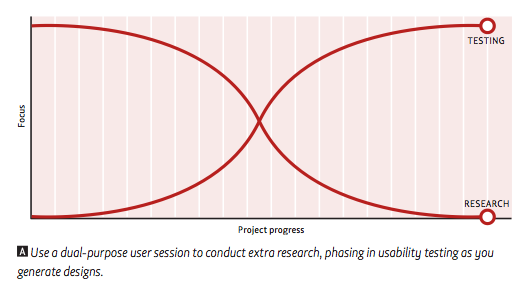
\includegraphics[width=120mm]{images/bowles_dualpurpose_testing.png}}
  \end{center}
  \caption{User session focus chart originally published in
    ``Undercover User Experience Design'', Bowles and Box \cite{bowles2011undercover}.}
  \label{bowles_dualpurpose_chart}
\end{figure}

\subsubsection{With students}

In the meetings with students, the questions asked predominantly revolved
around module allocation the University of York; it was important to
understand how they feel about the current state of module allocation to
ensure that the system improves the experience.

Students were asked to use a mockup of the application written in \gls{html}
and the researcher observed to discover the main areas of difficulty around
using web applications. Students were asked how and where they access to web,
to get an understanding of the environments this application might be used in.

% Discuss the results of the student interviews

\subsubsection{With staff}

I also spoke to departmental administrators, who will be responsible for setting up
the system. We discussed:

\begin{itemize}
  \item The idea of ``fairness''
  \item The user interface
  \item Administration
\end{itemize}

% Discuss the results of the staff interviews

\subsection{Web application frameworks}
\label{sec:webframeworks}

% Justifying a framework for this project

While it is possible to build a web application without using a framework,
there is no advantage to rewriting basic operations for this project. If the
system needed to operate at a scale or speed far beyond what these frameworks
were capable of, it is likely that the software would have to be built from
scratch to meet those requirements.

With the limited amount of time allocated to development and implementation,
it is sensible to spend a small amount of time choosing a framework to allow
more time to implement the system.

%   Could reference the Gantt chart (if it's included) here.

\subsubsection{Framework language}

% The programming language

The most important consideration when choosing a framework is the language it
is written in, as this defines, among other things, how easy the software will
be to maintain in the future.

% ColdFusion ML
%   - http://www.york.ac.uk/communications/websites/content/programming/cms-integration/
% Java
% PHP
%   - http://www.york.ac.uk/it-services/facilities/web/php/

There are three languages used for most web development at the University of
York. \emph{ColdFusion Markup Language} (CFML) is a language for creating web pages,
the most popular commercial implementation of which is Adobe ColdFusion.
ColdFusion is used widely across the University, including in applications
such as the ``People Directory'' search tool (shown in
Figure~\ref{yorkacuk_directory_search}) and online account management
facilities. \emph{Java} was used in the creation of the new Student Portal. A
\emph{PHP} service is offered by the University for users to deploy their PHP
applications.

\begin{lstlisting}[language=HTML]
<cfparam name="attributes.userid" type="string" default="unknown">
<h1>Hello, world</h1>
<cfoutput>
  <p>Welcome, #HTMLEditFormat(attributes.userid)#.</p>
</cfoutput>
\end{lstlisting}

In a presentation at \gls{oscon} in 2007 \cite{raible2007javawebframeworks},
Matt Raible compared several web frameworks written in Java; JavaServer Faces
(JSF), Spring MVC, Stripes, Struts 2, Tapestry and Wicket.

While there are a wide variety of Java web application frameworks available,
the University of York has decided to use Spring, an open source framework
developed by a division of VMware (a virtualisation software provider). The
Spring framework has a \gls{mvc} component, making it entirely suitable for
this project. As this is a framework \gls{itservices} has deployed and can
support, it makes little sense to choose anything else.

CFML is unsuitable for this project as it is primarily a markup language -- the
allocation logic behind the application would have to be implemented in a
programming language such as Java or Python. Using two languages to create
this application would needlessly increase the complexity of any maintenance.

% Ruby
% Python

Outside the University of York, popular web programming languages include
\emph{Ruby} and \emph{Python}.

% Rails guesses the model's attributes based on the database schema, whereas
% Django requires that the model's attributes be listed in the application, and
% the schema is then created.
% 
% There's a good comparison of Django and Rails which is quite methodical. In
% it, the authors note that equivalent applications took $\frac{2}{3}$ the time
% to be implemented in Django than Rails \cite{RailsDjangoComparison_2007}.
% 
% There's also a good comparison of the three big players that pretty much rules
% out CakePHP as being rubbish \cite{EvalWebDevFrameworks_2009}.

While Ruby or Python are both good languages for web application development,
neither is suitable for this project as they cannot be maintained by
\gls{itservices}.

\subsubsection{Summary}

% I chose a framework. It could be based on ColdFusion, Ruby or Python. Or
% something else entirely, even PHP or Java. But at the moment I'm not sure.

The framework chosen for this project was Spring MVC, written in Java.

% Because it'll be maintained by IT Services, primarily.

\subsection{Supporting software}

In addition to the web framework, there is a range of other software available
to support the creation of the application.

\subsubsection{Spring Roo}

Spring Roo is a tool created by SpringSource (the Spring development team) to
aid developers in creating Java web applications. It works by providing an
executable, \texttt{roo}, which generates ``application scaffolding''
programatically.

For example, inside Roo it is possible to run:

\begin{lstlisting}
project --topLevelPackage uk.ac.york.module_allocation
persistence setup --database MYSQL --provider HIBERNATE
entity --class ~.domain.Student
field string --fieldName username
\end{lstlisting}

These four lines of code generate a Java class representing a student, 500
lines of XML configuration files and 20 lines of application property files.

The major concern when considering a generation tool such as Roo is the
lock-in that it entails. However, Chapter 6 of the Roo reference documentation
\cite{RooReferenceDocs2011} is titled ``Removing Roo''. In it, the authors
note that a key part of the Roo mission statement was ``without compromising
engineering integrity or flexibility''. The developers provide a simple,
three-step guide to removing Roo from the project. If the future maintainers
of this software require that it not include Roo, it will be easy to remove.

The benefits that Roo provides in the short-term far outweigh the time that
might need to be spent removing it.

\subsubsection{Templating engines}

% Additionally: iText PDF, JExcel, Jasper Reports, and XSLT are all supported
% by Spring

There are many different templating engines that can be used as components of
a Java (in this case, Spring) project. Examples of commonly-used Java
templating software include \gls{jsp}, Tiles, Freemarker and Velocity.

% Plain old JSP

\gls{jsp} is a common language that is also used in Tiles. \gls{jsp} can be
used at a basic level to include dynamic elements in \gls{html}. The following
is an example of a \texttt{.jsp} file that outputs \gls{html} to the client:

\begin{lstlisting}[language=HTML]
<html>
  <h1>Welcome to the module allocation system, ${student_name}!</h1>
</html>
\end{lstlisting}

% Apache Tiles

Apache Tiles builds on just using \gls{jsp} markup by itself, by providing
other useful functions. Templates are written in the same language, but
developers can define `fragments' which are assembled when the page is
requested. The fragments (or tiles, which is where the software gets its name)
can be used to build up a page from its constituent parts. For example, it is
possible to define fragments for the page header and footer, to ensure they
are identical across every page. A template file may resemble the following,
where \texttt{header.jsp} and \texttt{footer.jsp} are files that contain the
site header and footer respectively:

\begin{lstlisting}[language=HTML]
<html>
  <tiles:insertTemplate path="/fragments/header.jsp" />
  <div id="container">
    <h1>This is the actual page content.</h1>
  </div>
  <tiles:insertTemplate path="/fragments/footer.jsp" />
</html>
\end{lstlisting}

% Freemarker

Freemarker is more complex than Tiles, offering functionality such as allowing
the developer to iterate over an array in the template file itself. This is
beneficial if the application requires functionality such as outputting lists
of elements:

\begin{lstlisting}[language=HTML]
<html>
  <#include "header.ftl" />
  <h1>Welcome to the module allocation system, ${student_name}!</h1>
  <p>These are the modules you have been allocated:</p>
  <ul>
  <#list modules as m>
    <li <#if m.level == "hard">class="hard"</#if>>${m.name} (${m.code})</li>
  </#list>
  </ul>
</html>
\end{lstlisting}

% Apache Velocity

Apache Velocity is similar to Freemarker, though the syntax appears more clear
and readable at a glance:

\begin{lstlisting}[language=HTML]
<html>
  #include("header.vm")
  <h1>Welcome to the module allocation system, $student_name!</h1>
  <p>These are the $modules.size() modules you have been allocated:</p>
  <ul>
  #foreach($m in $modules)
    <li>$m.name ($m.code)</li>
  #end
  </ul>
</html>
\end{lstlisting}

In his paper on enforcing separation between the model and the view, Parr
\cite{Parr2004templateengines} ranks Freemarker very poorly and Velocity more
favourably.

% StringTemplate

Parr has also created a templating engine, named StringTemplate, that enforces
separation of the model and the view. His paper articulates clearly why
enforcing the separation between model and view is a positive for a web
application, and his argument is convincing. As would be expected, his
templating engine is strict about applying the constraints he argues in favour
of in his paper.

% \subsubsection{Database thingys}

% EclipseLink or Hibernate

\subsection{Design decisions and visual appearance}

The application should be visually consistent with other University web
software to instill trust in the user.

\begin{figure}
  \begin{center}
    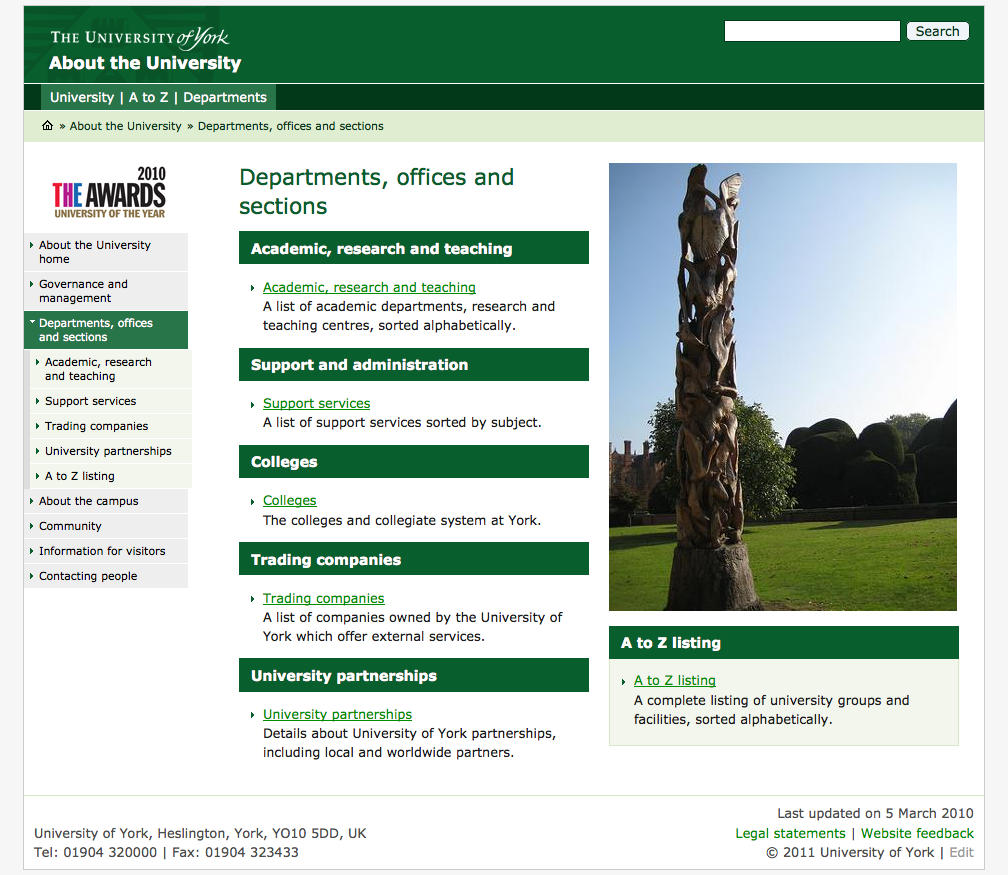
\includegraphics[width=160mm]{images/2011_11_06_yorkacuk.png}
  \end{center}
  \caption{A general page on the University site, using University colours.}
  \label{yorkacuk_general_page}
\end{figure}

\begin{figure}
  \begin{center}
    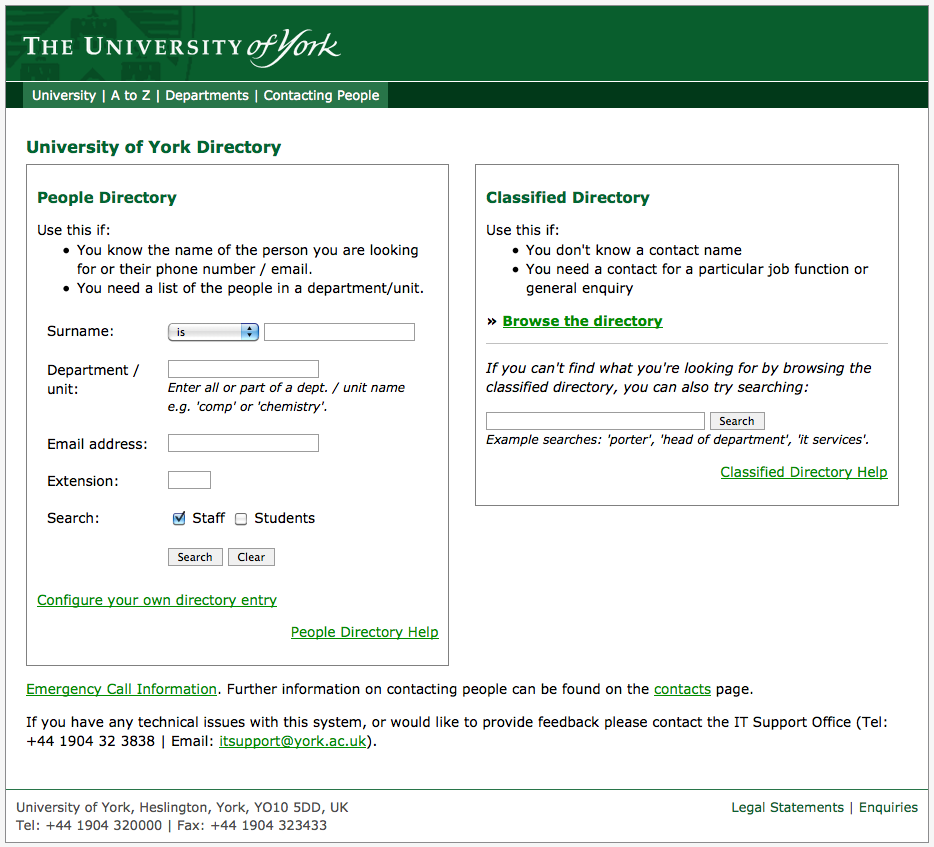
\includegraphics[width=160mm]{images/2011_11_06_yorkacuk_directory.png}
  \end{center}
  \caption{The University of York People Directory search tool.}
  \label{yorkacuk_directory_search}
\end{figure}

% Include screenshots of University software:
%   https://www.york.ac.uk/it-services/facilities/account/accounts
%   https://www.cs.york.ac.uk/submit/assessment/

One area that usability gains can be made are in relation to how the
application saves data. During one of the user research sessions, the
participant explained that while choosing optional modules during her first
year, she neglected to press that application's ``OK'' button and, unaware
that she had not submitted choices, was unable to take her preferred modules.

As an explicit ``Save'' button should be retained to reduce surprise and allow
the user to feel in control, the most sensible decision is to automatically
save user input periodically and notify users that their choices are being
saved. The submit button would save data in case of failure of the automatic
save mechanism.

\subsection{Accessibility}

% I could perhaps talk to Dave Swallow, CS.

Educational institutions such as the University of York are required by law to
ensure that web content is accessible to disabled users.

% http://www.york.ac.uk/communications/websites/policies/accessibility/
% http://www.york.ac.uk/communications/websites/content/accessibility/

\subsection{Interaction with other University software}

The system will be required to interact with \gls{sits}, as it is a centrally
maintained database that must always contain a true and accurate
representation of a student's data. Data stored in \gls{sits} is used in all
matters related to a student, including timetabling and room allocation.

This system will interact with \gls{sits} at two points:

\begin{enumerate}
  \item Module and student data must be imported during setup
  \item Student data must be exported after the allocation
\end{enumerate}

The import and setup will be performed by departmental administrators. This is
to reduce the workload on \gls{ssdt}, especially as administrators will be
required to tailor their setup after import.

For the pilot of this module allocation software, the export will be performed
manually by a member of \gls{ssdt}. They will perform a ``sanity check'' that
the data generated by this application seems accurate and will import the
data. If this application is evaluated successfully and maintained centrally,
it will not be feasible to import the data manually and some kind of automatic
import will have to be developed (Section~\ref{sec:autoexport}).

% Add notes from meeting with Matt

\subsection{Allocation algorithm}

Let's discuss the algorithm here.

\subsection{Issues arising during implementation}

% Discuss some of the _real_ issues of a _real_ project

One of the most positive aspects of undertaking this project was in fact one
of the most difficult -- that is, the project was undertaken very closely with
the University of York and as such relied on ``real'' stakeholders.

An issue arose fairly early in the project when it became clear that some
administrative staff (both IT support staff and those in the pilot
departments) would be away from work or leaving their jobs during the creation
of this application. This caused delays while the replacement staff had to be
brought up to speed on the background and current state of the project.

The issue was mitigated with the help of the \gls{aso}, which was responsible
for assisting with issues not directly related to implementation. The new or
replacement staff were then invited to group meetings so that they could keep
up to speed with recent developments and provide any necessary input.

% Also discuss how no technical people were involved early enough e.g. Andrew

% I was unable to respond to bugs as I couldn't have access to student data

\subsection{Testing}

How will the software be tested?

\subsection{Pilot by the Archaeology and History departments}

How did the pilot go?

\section{Further work}
\label{sec:furtherwork}

% A chapter describing possible ways in which your work could be continued or
% developed. Be imaginative but realistic.

We should probably ask departments what they'd like to see in the future.

If I didn't have time to implement a weighting system (rather than a simple,
plain ranking system) I could talk about that here.

\subsection{Automatic import and export}
\label{sec:autoexport}

The application could automatically import and export data.

\subsection{Expanding the use of the application}

The Chair of Board of Studies in Archaeology posed the question of whether
this application could be used to allow visiting students to select their
modules.

\section{Conclusions}
\label{sec:conclusions}

% This is similar to the abstract. The difference is that you should assume
% here that the reader of the conclusions has read the rest of the report.

It was a success. Well, hopefully.

\appendix

% What should go in an appendix? Screenshots? Code? Something else?

\newpage
\section{External links}

This appendix gives URLs to departments, offices or services mentioned
throughout the document.

University Teaching Committee sponsored this project on behalf of the
University of York:
\url{http://www.york.ac.uk/about/organisation/governance/sub-committees/teaching-committee/}

IT Services hosted and maintained the application once it had been created:
\url{http://www.york.ac.uk/it-services/}

I would like to make the code of this software available online, at
\url{https://github.com/alexmuller/york-allocation}.

\newpage
\section{Participant consent form}
\label{sec:consent}

All research participants (students and staff of the University of York)
signed the consent form shown in Figure~\ref{participantconsent} immediately
before their interview took place. This consent form is adapted from one made
available by Alistair Edwards for Computer Science students to use during
their projects. As of 5 November 2011, the original is available at
\url{http://www-users.cs.york.ac.uk/~alistair/projects/consent.html}.

In each case, the top half of the form was retained by the project author and
the second half was given to the participant in case they had any further
questions about the interview.

\begin{figure}[h]
  \begin{center}
    \fbox{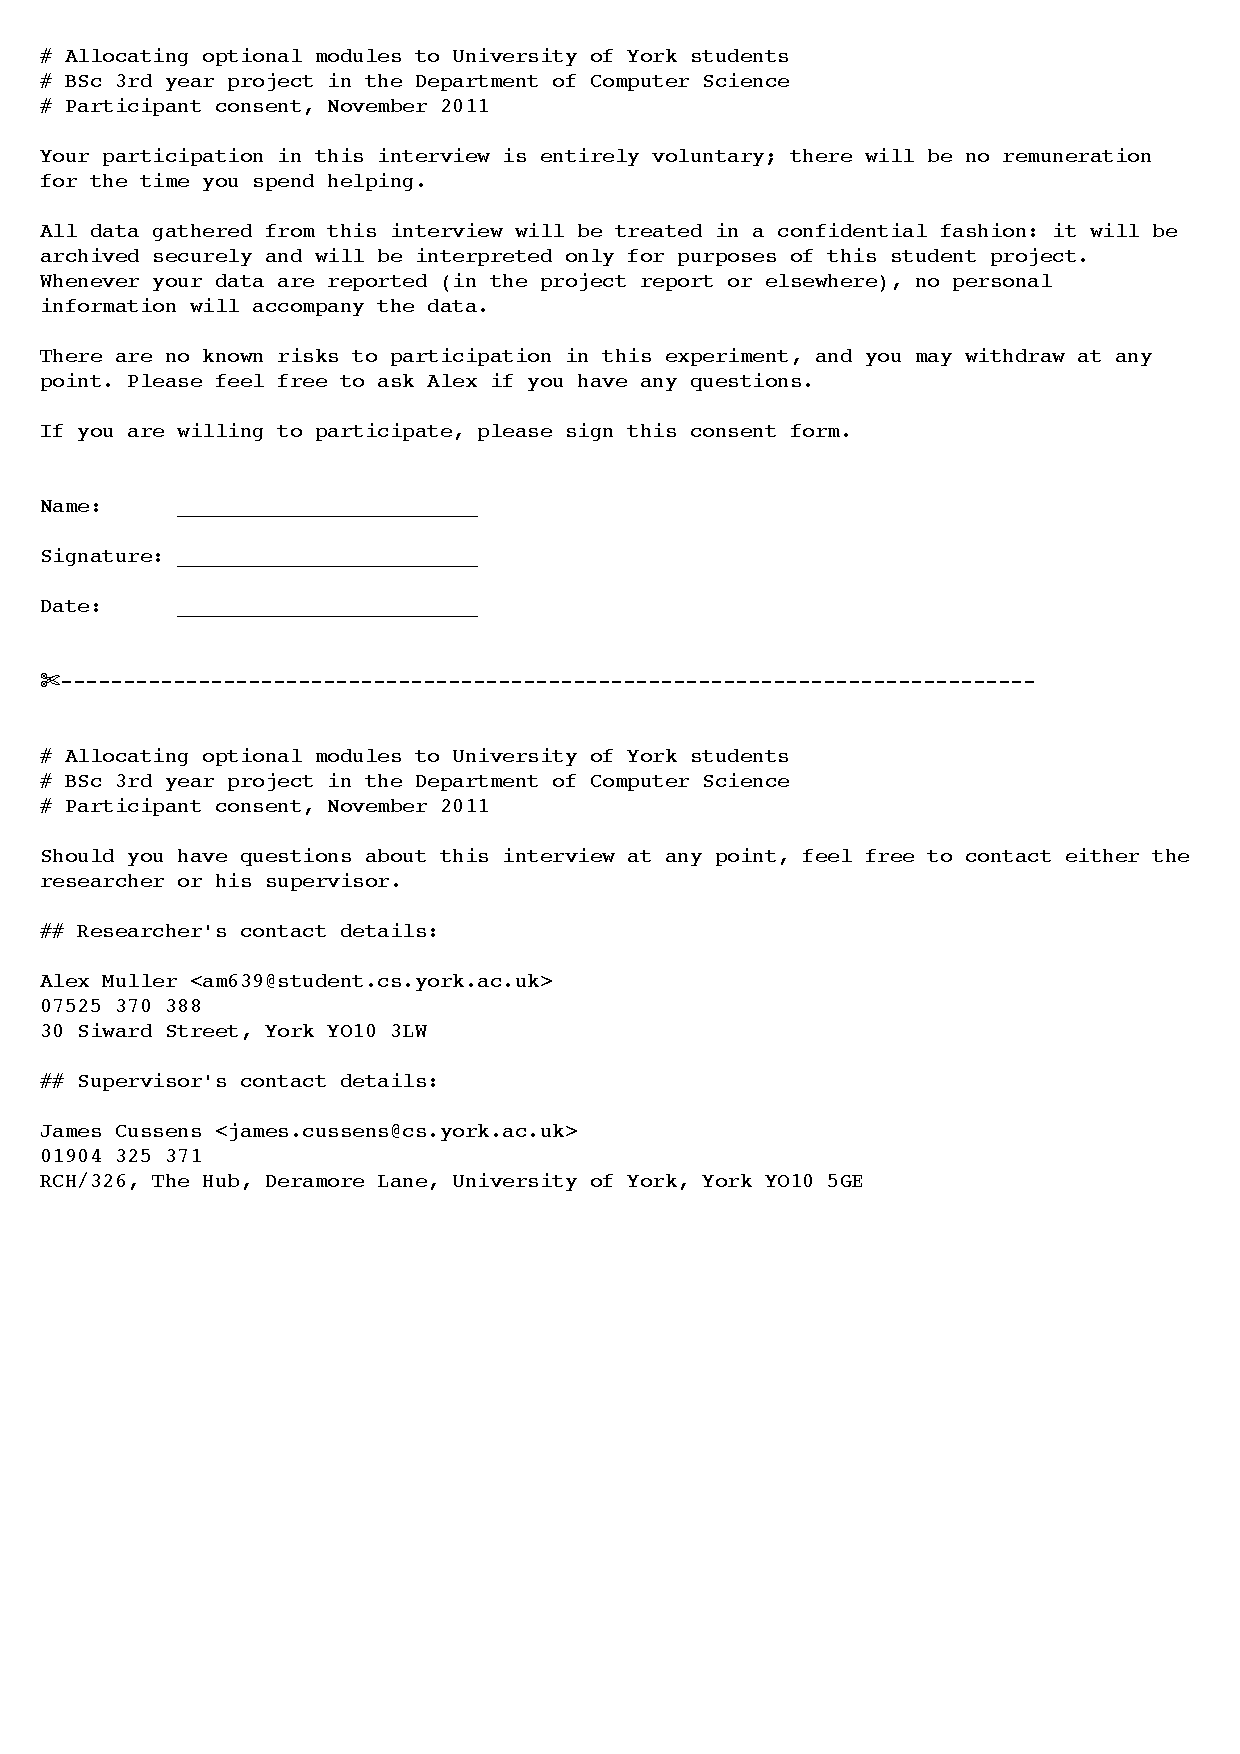
\includegraphics[width=140mm, trim=0 80mm 0 0]{images/consent.pdf}}
  \end{center}
  \caption{Participant consent form.}
  \label{participantconsent}
\end{figure}

\newpage
\printglossaries

\newpage
\bibliographystyle{references/IEEEtran.bst} % not just plain
\bibliography{references/references.bib}


\end{document}
